\subsection{Admin Module}
Το Admin Module είναι ένα σύνολο λειτουργιών που επιτρέπει έναν διαχειριστή να διαχειρίζεται με ευκολία την εφαρμογή. Στην παρούσα υλοποίηση το Admin Module έχει 2 διαφορετικές σελίδες - Components, το Κέντρο Ελέγχου και το Κέντρο Διαχείρισης Καταγραφών. Για να αποκτήσει πρόσβαση ένας χρήστης στις λειτουργίες του Admin Module, πρέπει να έχει κάνει Login και να είναι εξουσιοδοτημένος με τον ρόλο ADMIN, διαχειριστή. 

Το Κέντρο Ελέγχου είναι μια σελίδα που επιτρέπει την παρακολούθηση της κατάστασης της υγείας της εφαρμογής, προσφέρει στατιστικά των υπηρεσιών αλλά και του λειτουργικού που τρέχει η εφαρμογή αλλα παράλληλα προσφέρει και διαγνωστικά για να γνωρίζει ο διαχειριστής τι γίνεται ανά πάσα στιγμή στην εφαρμογή αυτήν όπως φαίνεται στις εικόνες \ref{layout:admin_cc_1} και \ref{layout:admin_cc_2}. 

Αποτελείται από πολλά διαφορετικά Components τα οποία ενημερώνονται ανάλογα με τον τύπο των δεδομένων που προσφέρουν ανά μισό, δύο και ανά πέντε δευτερόλεπτα με την χρήση WebSockets μέσο του Spring Boot Actuator έτσι ώστε η εικόνα που βλέπει ο διαχειριστής να αντικατοπτρίζει πάντα την κατάσταση της εφαρμογής εκείνη την χρονική στιγμή.

Το Κέντρο Διαχείρισής Καταγραφών είναι στην ουσία ένας διαδραστικός πίνακας που επιτρέπει στον διαχειριστή να αλλάζει τα επίπεδα καταγραφής διάφορων υπηρεσιών μέσα στον Server. Τα επίπεδα καταγραφής ορίζουν τι πληροφορίες θα δίνει η κάθε υπηρεσία. Το επίπεδο καταγραφής ERROR για παράδειγμα καταγράφει μόνο τα μηνύματα σφαλμάτων στο αρχείο καταγραφής της υπηρεσίας, ενώ το επίπεδο καταγραφής WARNING καταγράφει και τα μηνύματα σφαλμάτων αλλά και τα μηνύματα προειδοποιήσεων. Αυτό είναι πολύ χρήσιμο όταν χρησιμοποιείται σε συνδυασμό με μια υπηρεσία διαχείρισης καταγραφών όπως η Logstash για παράδειγμα. Με αυτόν τον τρόπο ο διαχειριστής δεν χρειάζεται να έχει φυσική πρόσβαση στο μηχάνημα που τρέχει την εφαρμογή για να μπορεί να δει τα αρχεία καταγραφής παρά μόνο να μπει στην υπηρεσία διαχείρισης καταγραφών και να βρει ότι χρειάζεται από εκεί.

Ο πίνακας του Κέντρου Διαχείρισής Καταγραφών φαίνεται στην εικόνα \ref{layout:admin_l}. Η συγκεκριμένη εικόνα τραβήχτηκε κατά την ανάπτυξη της εφαρμογής και δείχνει ότι το κεντρικό επίπεδο καταγραφών ROOT είναι ορισμένο στο DEBUG που σημαίνει ότι καταγράφει ακόμα και μηνύματα διαγνωστικών με κάποιες εξαιρέσεις που έχουν οριστεί σε επίπεδο WARNING για να μην υπερφορτώσουν τα αρχεία καταγραφής με περιττές πληροφορίες.

\begin{figure}[H]
  \centering
  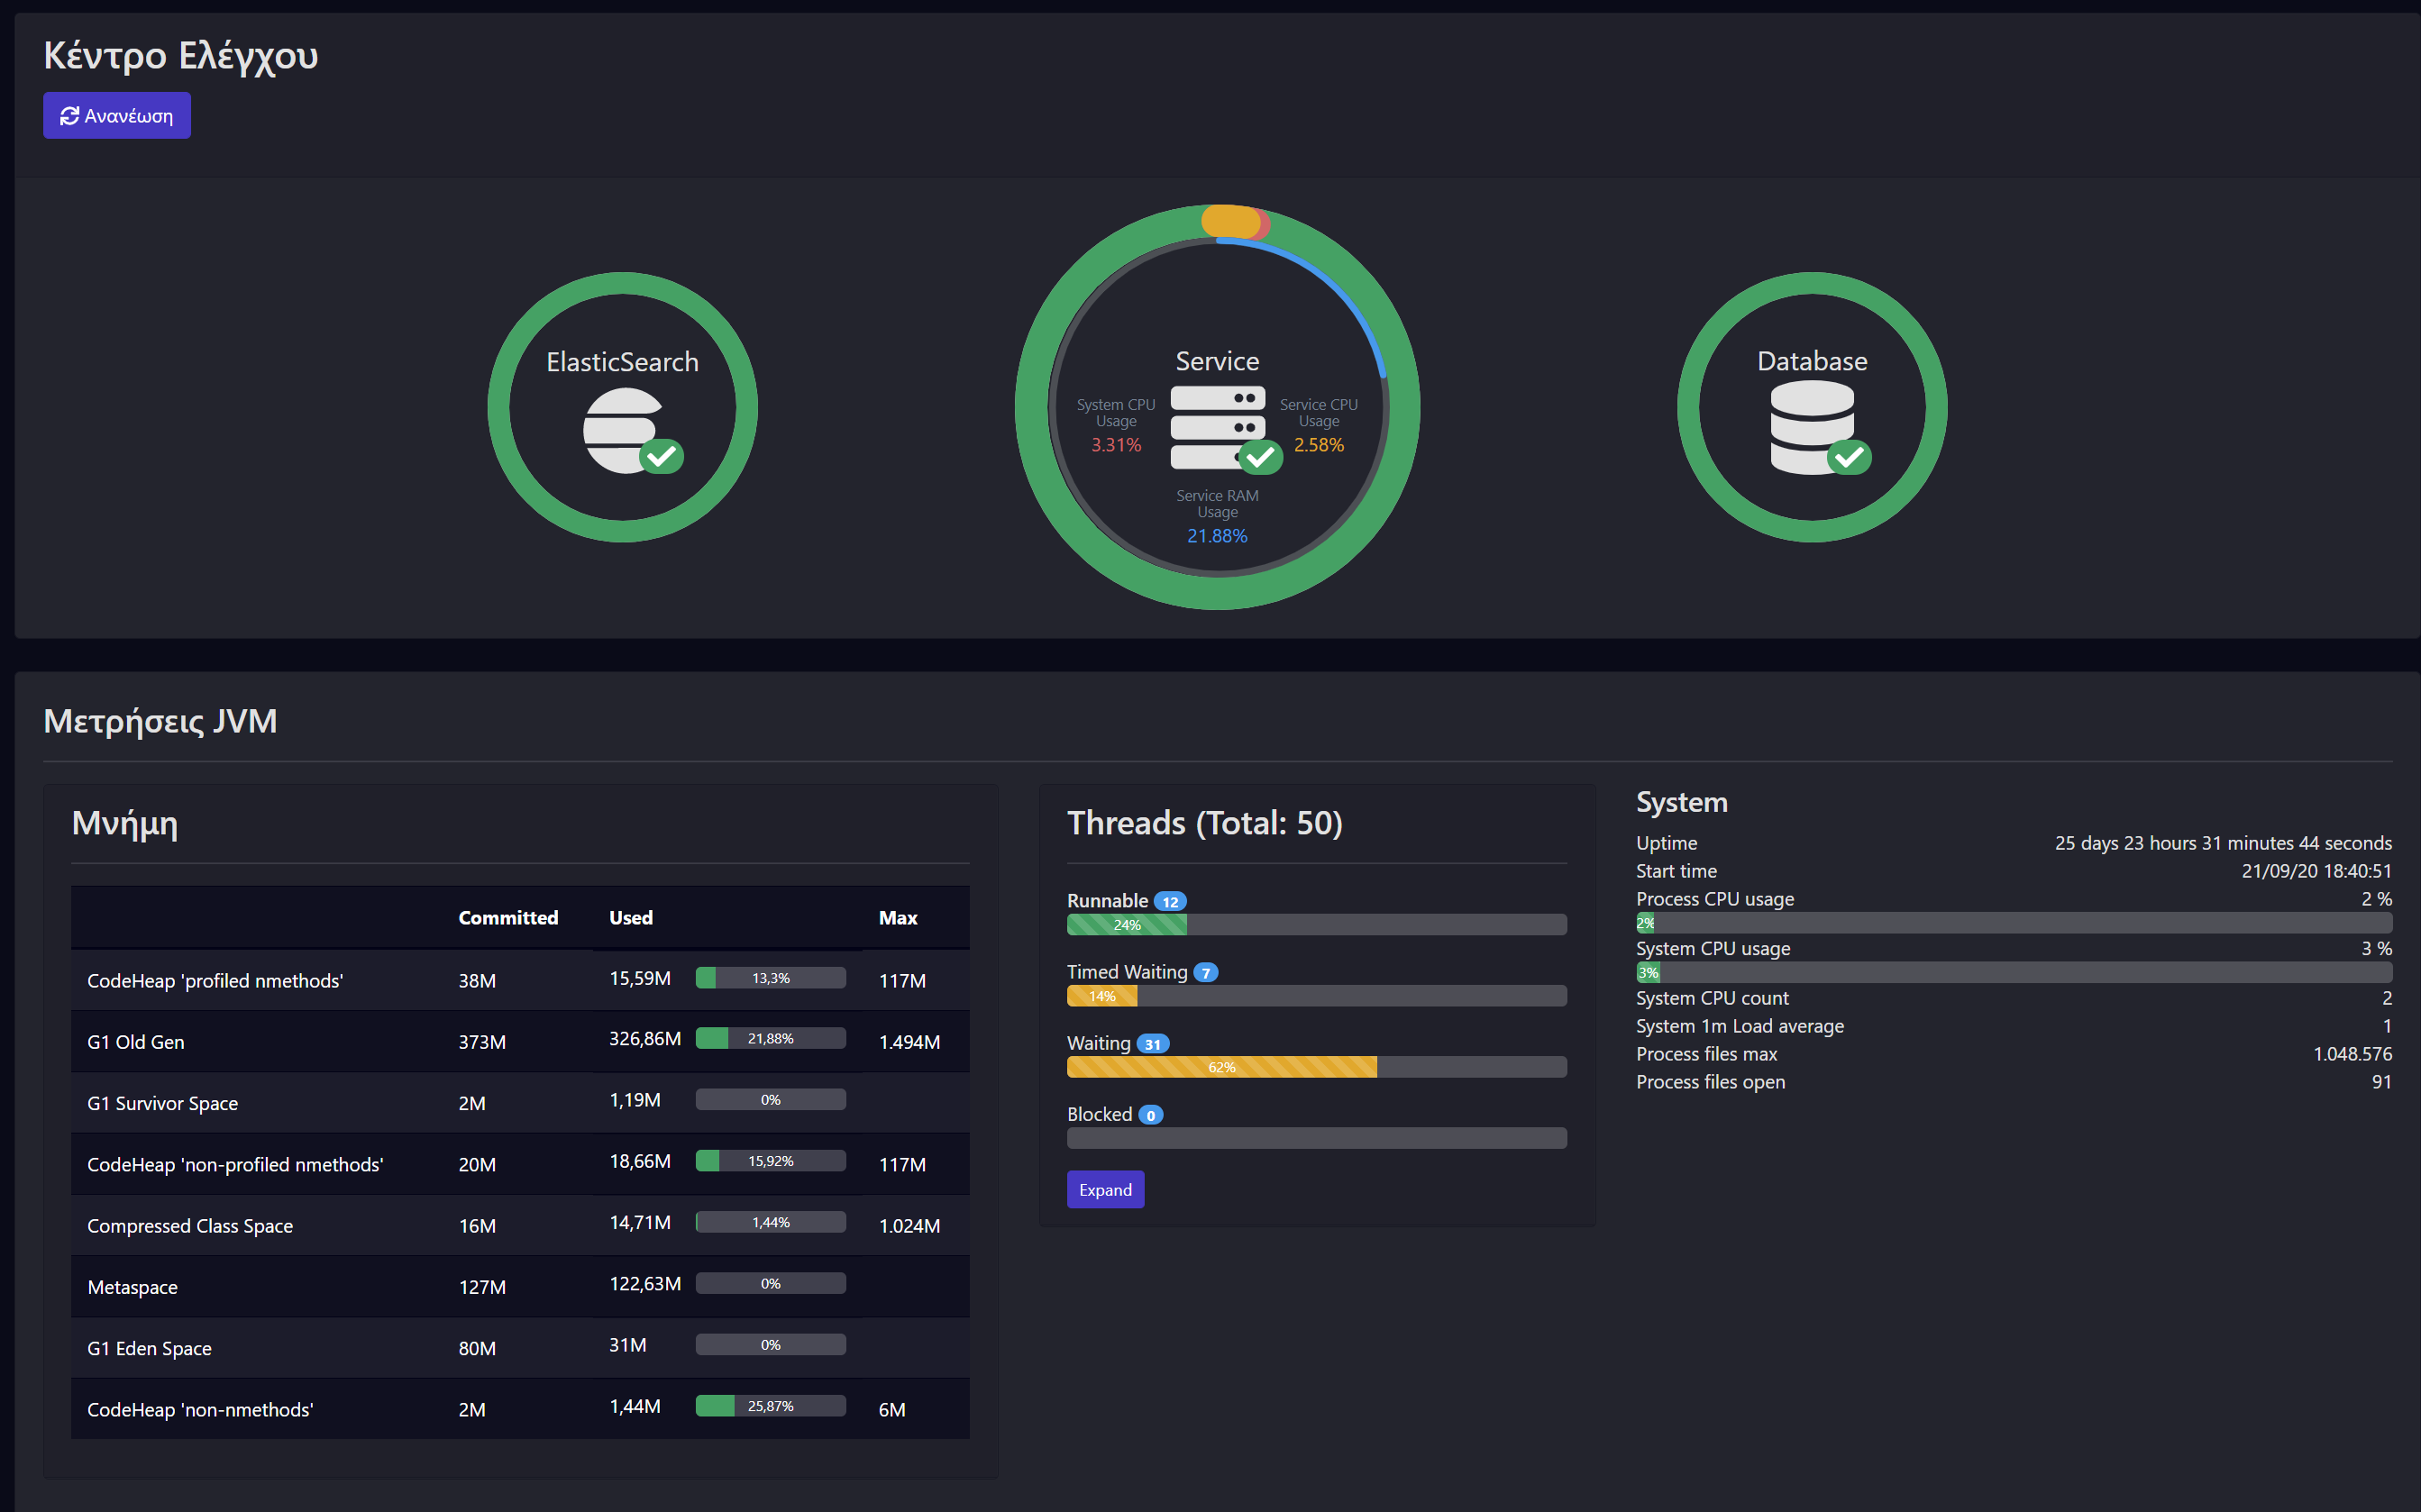
\includegraphics[width=145mm]{Chapters/5 - Architecture/Client/Images/admin_control_center.png}
  \caption{Κέντρο Ελέγχου}
  \label{layout:admin_cc_1}
\end{figure}
\begin{figure}[H]
  \centering
  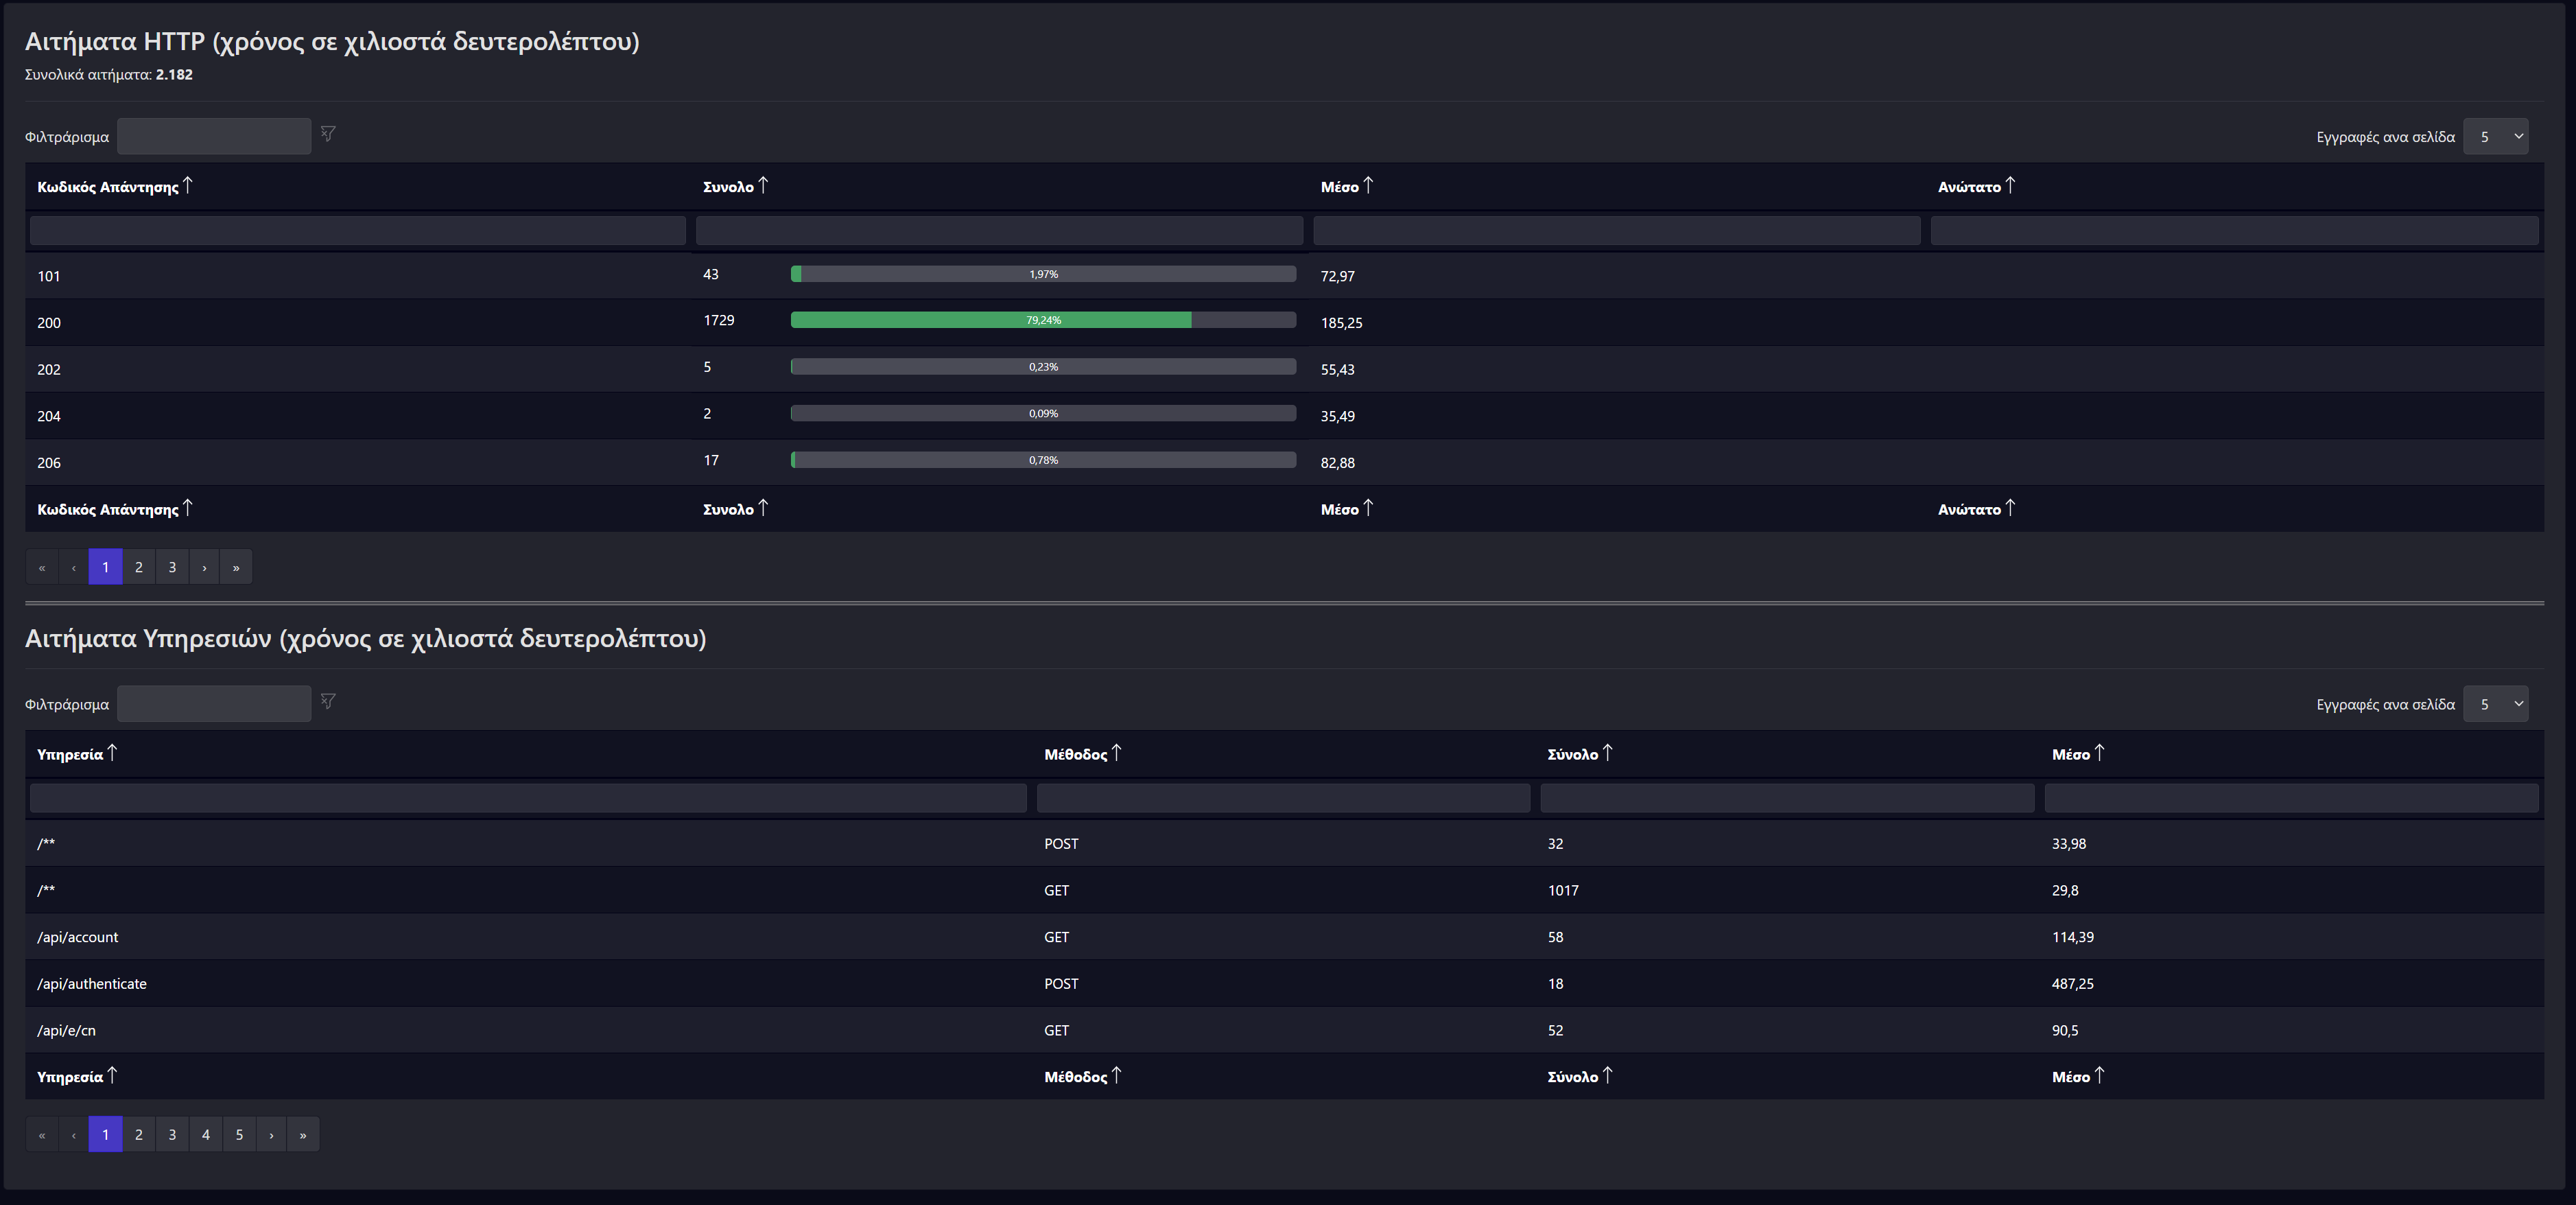
\includegraphics[width=145mm]{Chapters/5 - Architecture/Client/Images/admin_control_center_2.png}
  \caption{Κέντρου Ελέγχου - συνέχεια}
  \label{layout:admin_cc_2}
\end{figure}
\begin{figure}[H]
  \centering
  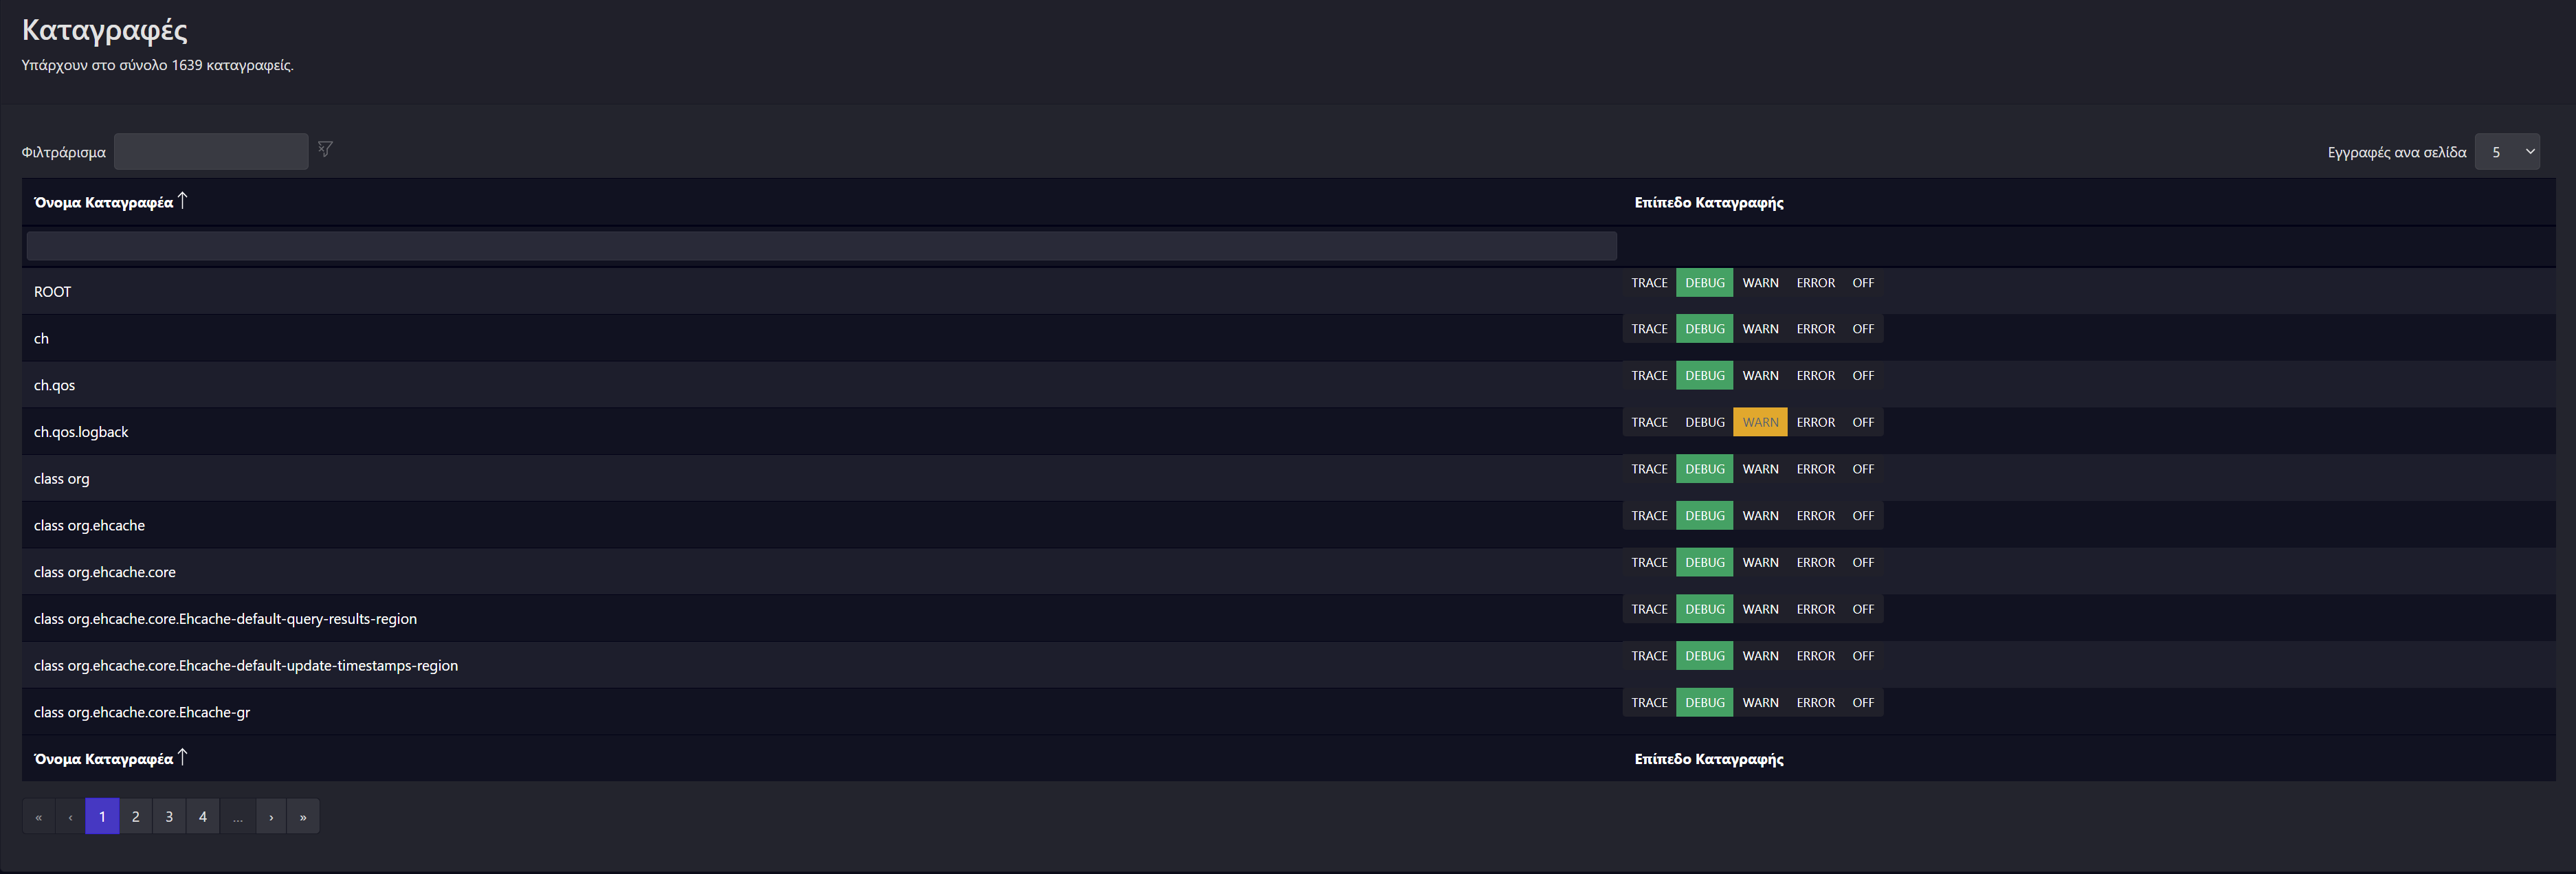
\includegraphics[width=145mm]{Chapters/5 - Architecture/Client/Images/admin_l.png}
  \caption{Κέντρο Διαχείρισής Καταγραφών}
  \label{layout:admin_l}
\end{figure}